\documentclass{beamer}

\usepackage[version=4]{mhchem}  
\usepackage{tikz}
\usepackage{caption}
\usepackage{gensymb}
% \usepackage{polyglossia}
\usepackage{subcaption}

% \setmainlanguage{lithuanian}
\usepackage[
  backend=biber,
  style=numeric,
  sorting=ynt
]{biblatex}

\addtobeamertemplate{navigation symbols}{}{%
  \usebeamerfont{footline}%
  \usebeamercolor[fg]{footline}%
  \hspace{1em}%
  \insertframenumber/\inserttotalframenumber
}

\bibliography{bibliografija}

\usetheme{Copenhagen}

\setbeamertemplate{caption}[numbered]
\setbeamertemplate{headline}{}

\date{2025}

\title[]{Modelling the mixing of reagents in YAG reaction}

\author[Arnas Vaicekauskas]
{
    A.~Vaicekauskas\inst{1}\\ 
    \small Supervisor: Asist. Dr. R.~Astrauskas\inst{1}
}

\institute[MIF]
{
  \inst{1}
  Faculty of Mathematics and Informatics\\
  Vilnius University
}

\begin{document}

\frame{\titlepage}

\frame{
  \tableofcontents[currentsubsection,subsectionstyle=show]
}

\section{Introduction}

\begin{frame}
  \frametitle{YAG -- yttrium aluminum garnet}

  This material has many applications, one of them -- lasers

  \begin{figure}
    \centering
    \begin{subfigure}[t]{0.45\linewidth}
      \includegraphics[width=\linewidth]{assets/NdYAG.png}
      \caption{Nd:YAG -- YAG crystals doped with neodymium ions}
    \end{subfigure}
    \hfill
    \begin{subfigure}[t]{0.45\linewidth}
      \includegraphics[width=\linewidth]{assets/NdYAG-laser.jpg}
      \caption{Nd:YAG laser}
    \end{subfigure}
  \end{figure}
\end{frame}

\begin{frame}
  \frametitle{YAG synthesis reaction}

  Research object -- YAG synthesis reaction:

  \centering
  \begin{align*}
    \ce{3Y_2O_3 + 5Al_2O_3 -> 2Y_3Al_5O_{12}}
  \end{align*}    

  \begin{itemize}
    \item The reaction takes place by heating a homogeneous mixture of yttrium and aluminum oxides at a high temperature ($1000-1600$ C\degree)
    \item The reaction duration can reach several hours
    \item In practice, the reagents are periodically mixed -- this accelerates the reaction
  \end{itemize}
\end{frame}

\section{Motivation for research}

\begin{frame}
  \frametitle{Motivation for research}

  \begin{itemize}
    \item Modeling material mixing can help to understand the processes occurring during the YAG reaction, which cannot be physically investigated due to the environmental conditions required for the reaction
    \item The efficiency of computer models allows simulating the YAG synthesis reaction much faster and more cheaply than physical experiments in a laboratory
  \end{itemize}
\end{frame}

\section{Research aim}
\begin{frame}
  \frametitle{Research aim}

  \begin{enumerate}
    \item Determine whether it is sufficient to model the reaction in a small spatial region when mixing materials
    \item Determine how the reaction duration depends on the mixing time
  \end{enumerate}
\end{frame}

\section{Tools and methods}

\begin{frame}
  \frametitle{Tools and methods}
  \begin{itemize}
    \item Graphical results were created and calculations performed using the \textit{Python} programming language and the \textit{NumPy}, \textit{Matplotlib}, and \textit{SciPy} packages
    \item An equation system solver was implemented, based on the explicit FTCS method (\textit{explicit forward time centered space})
  \end{itemize}
\end{frame}

\section{Mathematical model}

\subsection{Reaction-diffusion system}

\begin{frame}
  \frametitle{Mathematical reaction-diffusion system}

  Reaction-diffusion system describing the YAG synthesis reaction:
  
  \begin{align*}
    \frac{\partial c_1}{\partial t} & =-3kc_1c_2+D\left(\frac{\partial^2c_1}{\partial x^2}+\frac{\partial^2c_1}{\partial y^2}\right) \\
    \frac{\partial c_2}{\partial t} & =-5kc_1c_2+D\left(\frac{\partial^2c_2}{\partial x^2}+\frac{\partial^2c_2}{\partial y^2}\right)\\
    \frac{\partial c_3}{\partial t} & =2kc_1c_2\\
    (x, y, t)&\in(0, W)\times(0, H)\times[0, T]
  \end{align*}

\end{frame}

\subsection{Initial and boundary conditions}

\begin{frame}
  \frametitle{Initial and boundary conditions}

  \begin{figure}
    \centering
    \begin{subfigure}[t]{0.55\linewidth}
      \includegraphics[width=\linewidth]{assets/initial-model.png}
      \caption{Idealized model of the homogenous mixture}
    \end{subfigure}
    \hfill
    \begin{subfigure}[t]{0.35\linewidth}
      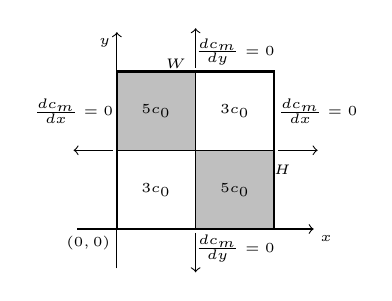
\begin{tikzpicture}[scale=1.0]
        \tiny
        \draw[fill=white] (0,0) rectangle (1,1);
        \draw[fill=white] (1,1) rectangle (2,2);
        \draw[fill=gray!50] (0,1) rectangle (1,2);
        \draw[fill=gray!50] (1,0) rectangle (2,1);

        % Draw the boundary of the square
        \draw[thick] (0,0) rectangle (2,2);

        % Draw axes
        \draw[->] (-0.5, 0) -- (2.5, 0) node[anchor=north west] {$x$};
        \draw[->] (0, -0.5) -- (0, 2.5) node[anchor=north east] {$y$};

        % Mark the origin
        \node[anchor=north east] at (0,0) {$(0, 0)$};

        % Mark the side length
        \draw[-] (2,0) -- (2,2);
        \draw[-] (0,2) -- (2,2);

        \node at (2.1, 0.75) {$H$};
        \node at (0.75, 2.1) {$W$};
        
        \draw (0.5, 1.5) node[anchor=center] {$5c_0$};
        \draw (1.5, 0.5) node[anchor=center] {$5c_0$};
        \draw (1.5, 1.5) node[anchor=center] {$3c_0$};
        \draw (0.5, 0.5) node[anchor=center] {$3c_0$};

        % boundary conditions
        \draw[->] (-0.05,1) -- (-0.55,1);
        \node at (-0.55, 1.5) {$\frac{dc_m}{dx} = 0$};

        \draw[->] (2.05,1) -- (2.55,1);
        \node at (2.55, 1.5) {$\frac{dc_m}{dx} = 0$};

        \draw[->] (1, -0.05) -- (1, -0.55);
        \node at (1.5, -0.25) {$\frac{dc_m}{dy} = 0$};

        \draw[->] (1, 2.05) -- (1, 2.55);
        \node at (1.5, 2.25) {$\frac{dc_m}{dy} = 0$};

      \end{tikzpicture}
      \caption{Initial and boundary conditions of the model.}
      \label{initial-boundary-condition}
    \end{subfigure}
  \end{figure}
\end{frame}

% \subsection{Stabilumo sąlyga}

% \begin{frame}
%     \frametitle{Stabilumo sąlyga}
%     Galima parodyti, kad skaitinis sprendinys bus stabilus tada, kai tenkinama ši nelygybė:
%     \begin{align*}
%         \Delta t \leqslant \left(15kc_0+2D\left((\Delta x)^{-2}+(\Delta y)^{-2}\right)\right)^{-1}
%     \end{align*}
%     Čia $k$ - reakcijos greitis, $D$ - difuzijos konstanta, $\Delta x, \Delta y$ - diskretūs erdvės žingsniai, $c_0$ - pradinių medžiagų koncentracijų didžiausias bendras daliklis.
% \end{frame}

\subsection{Reaction-diffusion model results}

\begin{frame}
  \frametitle{Reaction-diffusion model results}

  Model evolution over time with initial and boundary conditions \eqref{initial-boundary-condition}
  \centering
  \includegraphics[width=12cm]{assets/example-0.png} \\ 
  \includegraphics[width=12cm]{assets/example-2.png}

\end{frame}

\section{Mixing models}
\subsection{Reaction stopping condition}

\begin{frame}
  \frametitle{Reaction stopping condition}

  \centering
  \begin{figure}
    \includegraphics[width=0.6\linewidth]{assets/stop.png}
    \caption{Amount of the first substance as a function of time}
  \end{figure}

  The reaction is stopped when the amount of the first two substances in the system reaches 3\% of the initial amount.

\end{frame}

\subsection{Random mixing}

\begin{frame}
\frametitle{Random mixing}
\begin{figure}
\centering
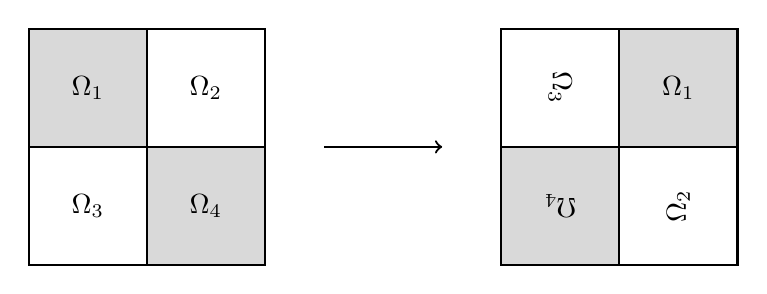
\begin{tikzpicture}[scale=1.5]

    \fill[gray!30] (0,1) rectangle (1, 2);
    \fill[gray!30] (1,0) rectangle (2, 1);

    % Original Grid
    \draw[thick] (0,0) rectangle (2,2);
    \draw[thick] (1,0) -- (1,2);
    \draw[thick] (0,1) -- (2,1);

    \node at (0.5,1.5) {$\Omega_1$};
    \node at (1.5,1.5) {$\Omega_2$};
    \node at (0.5,0.5) {$\Omega_3$};
    \node at (1.5,0.5) {$\Omega_4$};

    % Arrow
    \draw[->, thick] (2.5,1) -- (3.5,1);

    % Transformed Grid
    \begin{scope}[shift={(4,0)}]

        \fill[gray!30] (0,0) rectangle (1, 1);
        \fill[gray!30] (1,1) rectangle (2, 2);

        \draw[thick] (0,0) rectangle (2,2);
        \draw[thick] (1,0) -- (1,2);
        \draw[thick] (0,1) -- (2,1);

        \node at (0.5,1.5) {\rotatebox{270}{$\Omega_3$}}; % Rotated 180° horizontally
        \node at (1.5,1.5) {$\Omega_1$};             % No change
        \node at (0.5,0.5) {\rotatebox{180}{$\Omega_4$}}; % Upside down
        \node at (1.5,0.5) {\rotatebox{90}{$\Omega_2$}};  % 90° rotation
    \end{scope}
\end{tikzpicture}
\caption{During random mixing, the reaction space regions are randomly rotated and swapped.}
\label{random-mix}
\end{figure}
\end{frame}

\subsection{Random Mixing Results}
\begin{frame}
  \frametitle{Random Mixing Results}
  \begin{figure}
    \centering
    \includegraphics[width=12cm]{assets/random-mix-example-c0-1.png} \\
    \includegraphics[width=12cm]{assets/random-mix-example-c2-1.png}
    \caption{Model evolution over time with initial and boundary conditions \eqref{initial-boundary-condition}, using the random mixing model \eqref{random-mix}.}
  \end{figure}
\end{frame}

\begin{frame}
  \frametitle{Random Mixing Results}
  \begin{figure}
    \centering
    \includegraphics[width=7cm]{assets/bad-mix-qnt-compare-1.png}
    \caption{Problem of the random mixing model \eqref{random-mix} - it can significantly extend the reaction end time. The effect of such a model needs to be measured through statistical testing or brute force.}
  \end{figure}
\end{frame}

\subsection{Perfect mixing}
\begin{frame}
\frametitle{Perfect mixing}
\begin{figure}
\centering
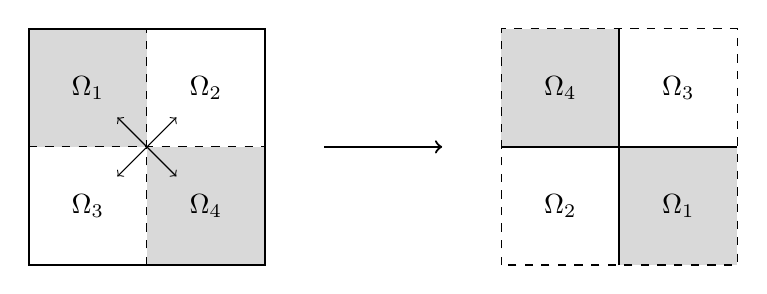
\begin{tikzpicture}[scale=1.5]
    % Original Grid
    \fill[gray!30] (0,1) rectangle (1, 2);
    \fill[gray!30] (1,0) rectangle (2, 1);
    \draw[<->] (0.75,0.75) -- (1.25,1.25);
    \draw[<->] (1.25,0.75) -- (0.75,1.25);
    \draw[thick] (0,0) rectangle (2,2);
    \draw[dashed] (1,0) -- (1,2);
    \draw[dashed] (0,1) -- (2,1);

    \node at (0.5,1.5) {$\Omega_1$};
    \node at (1.5,1.5) {$\Omega_2$};
    \node at (0.5,0.5) {$\Omega_3$};
    \node at (1.5,0.5) {$\Omega_4$};

    % Arrow
    \draw[->, thick] (2.5,1) -- (3.5,1);

    % Transformed Grid
    \begin{scope}[shift={(4,0)}]
        \fill[gray!30] (0,1) rectangle (1, 2);
        \fill[gray!30] (1,0) rectangle (2, 1);
        
        \draw[dashed] (0,0) rectangle (2,2);
        \draw[thick] (1,0) -- (1,2);
        \draw[thick] (0,1) -- (2,1);

        \node at (0.5,1.5) {$\Omega_4$};
        \node at (1.5,1.5) {$\Omega_3$};
        \node at (0.5,0.5) {$\Omega_2$};
        \node at (1.5,0.5) {$\Omega_1$};
    \end{scope}
\end{tikzpicture}
\caption{During perfect mixing, the reaction space regions are swapped diagonally, thus maximizing the reaction rate.}
\label{perfect-mix}
\end{figure}
\end{frame}

\subsection{Perfect Mixing Results}
\begin{frame}
\frametitle{Perfect Mixing Results}
\begin{figure}
\centering
\includegraphics[width=7cm]{assets/optimal-mix-qnt-1.png}
\caption{Perfect mixing is deterministic and more realistically reflects the consequences of mixing.}
\end{figure}
\end{frame}

\subsection{Perfect Mixing Model for Larger Spaces}
\begin{frame}
    \frametitle{Mixing in a Larger Space}
    \begin{figure}
    \centering
    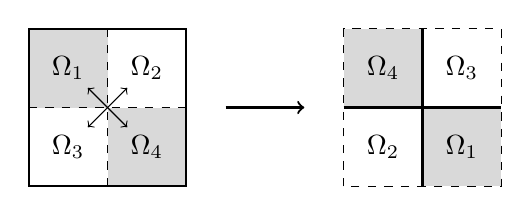
\begin{tikzpicture}
      \fill[gray!30] (0,1) rectangle (1, 2);
    \fill[gray!30] (1,0) rectangle (2, 1);
    \draw[<->] (0.75,0.75) -- (1.25,1.25);
    \draw[<->] (1.25,0.75) -- (0.75,1.25);
    \draw[thick] (0,0) rectangle (2,2);
    \draw[dashed] (1,0) -- (1,2);
    \draw[dashed] (0,1) -- (2,1);

    \node at (0.5,1.5) {$\Omega_1$};
    \node at (1.5,1.5) {$\Omega_2$};
    \node at (0.5,0.5) {$\Omega_3$};
    \node at (1.5,0.5) {$\Omega_4$};

    % Arrow
    \draw[->, thick] (2.5,1) -- (3.5,1);

    % Transformed Grid
    \begin{scope}[shift={(4,0)}]
        \fill[gray!30] (0,1) rectangle (1, 2);
        \fill[gray!30] (1,0) rectangle (2, 1);
        
        \draw[dashed] (0,0) rectangle (2,2);
        \draw[thick] (1,0) -- (1,2);
        \draw[thick] (0,1) -- (2,1);

        \node at (0.5,1.5) {$\Omega_4$};
        \node at (1.5,1.5) {$\Omega_3$};
        \node at (0.5,0.5) {$\Omega_2$};
        \node at (1.5,0.5) {$\Omega_1$};
    \end{scope}
    \end{tikzpicture}
    \vfill
    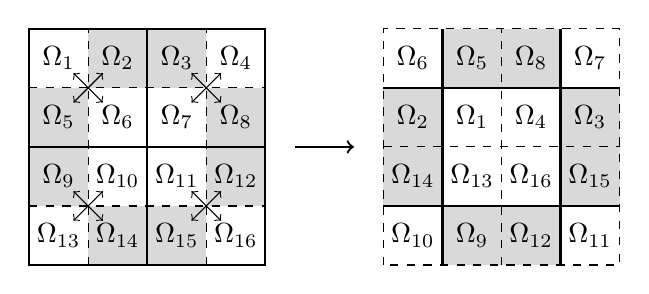
\begin{tikzpicture}[scale=0.75]
        % Original Grid
    
        \fill[gray!30] (1, 0) rectangle (3, 1);
        \fill[gray!30] (1, 3) rectangle (3, 4);
    
        \fill[gray!30] (0, 1) rectangle (1, 3);
        \fill[gray!30] (3, 1) rectangle (4, 3);
    
        \draw[thick] (0,0) rectangle (2,2);
        \draw[thick] (0,2) rectangle (2,4);
        \draw[thick] (2,0) rectangle (4,2);
        \draw[thick] (2,2) rectangle (4,4);
        \draw[dashed] (1,0) -- (1,4);
        \draw[dashed] (0,1) -- (4,1);
        \draw[dashed] (3,0) -- (3,4);
        \draw[dashed] (0,3) -- (4,3);
    
        \draw[<->] (0.75,0.75) -- (1.25,1.25);
        \draw[<->] (1.25,0.75) -- (0.75,1.25);
    
        \draw[<->] (2.75,0.75) -- (3.25,1.25);
        \draw[<->] (3.25,0.75) -- (2.75,1.25);
    
        \draw[<->] (0.75,2.75) -- (1.25,3.25);
        \draw[<->] (1.25,2.75) -- (0.75,3.25);
    
        \draw[<->] (2.75,2.75) -- (3.25,3.25);
        \draw[<->] (3.25,2.75) -- (2.75,3.25);
    
        \node at (0.5,3.5) {$\Omega_1$};
        \node at (1.5,3.5) {$\Omega_2$};
        \node at (0.5,2.5) {$\Omega_5$};
        \node at (1.5,2.5) {$\Omega_6$};
    
        \node at (2.5,3.5) {$\Omega_3$};
        \node at (3.5,3.5) {$\Omega_4$};
        \node at (2.5,2.5) {$\Omega_7$};
        \node at (3.5,2.5) {$\Omega_8$};
    
        \node at (0.5,1.5) {$\Omega_9$};
        \node at (1.5,1.5) {$\Omega_{10}$};
        \node at (0.5,0.5) {$\Omega_{13}$};
        \node at (1.5,0.5) {$\Omega_{14}$};
    
        \node at (2.5,1.5) {$\Omega_{11}$};
        \node at (3.5,1.5) {$\Omega_{12}$};
        \node at (2.5,0.5) {$\Omega_{15}$};
        \node at (3.5,0.5) {$\Omega_{16}$};
    
        % Arrow
        \draw[->, thick] (4.5,2) -- (5.5,2);
    
        % Transformed Grid
        \begin{scope}[shift={(6,0)}]
            \fill[gray!30] (1, 0) rectangle (3, 1);
            \fill[gray!30] (1, 3) rectangle (3, 4);
    
            \fill[gray!30] (0, 1) rectangle (1, 3);
            \fill[gray!30] (3, 1) rectangle (4, 3);
    
            \draw[dashed] (0,0) rectangle (4,4);
    
            \draw[dashed] (2,0) -- (2,4);
            \draw[dashed] (0,2) -- (4,2);
    
            \draw[thick] (1,0) -- (1,4);
            \draw[thick] (0,1) -- (4,1);
            \draw[thick] (3,0) -- (3,4);
            \draw[thick] (0,3) -- (4,3);
    
            \node at (0.5,3.5) {$\Omega_6$};
            \node at (1.5,3.5) {$\Omega_5$};
            \node at (0.5,2.5) {$\Omega_2$};
            \node at (1.5,2.5) {$\Omega_1$};
    
            \node at (2.5,3.5) {$\Omega_8$};
            \node at (3.5,3.5) {$\Omega_7$};
            \node at (2.5,2.5) {$\Omega_4$};
            \node at (3.5,2.5) {$\Omega_3$};
    
            \node at (0.5,1.5) {$\Omega_{14}$};
            \node at (1.5,1.5) {$\Omega_{13}$};
            \node at (0.5,0.5) {$\Omega_{10}$};
            \node at (1.5,0.5) {$\Omega_{9}$};
    
            \node at (2.5,1.5) {$\Omega_{16}$};
            \node at (3.5,1.5) {$\Omega_{15}$};
            \node at (2.5,0.5) {$\Omega_{12}$};
            \node at (3.5,0.5) {$\Omega_{11}$};
        \end{scope}
    \end{tikzpicture}
    \caption{The perfect mixing model for a larger space is analogous to the model \eqref{perfect-mix}, replicated using a mirror principle.}
    \label{large-perfect-mix}
\end{figure}
\end{frame}

\begin{frame}
  \frametitle{Perfect Mixing Results}

  \begin{figure}
    \centering
    \begin{subfigure}[t]{0.45\linewidth}
      \includegraphics[width=\linewidth]{assets/mix-end-1.png}
      \caption{Smaller reaction space. \label{fig:perfect-small}}
    \end{subfigure}
    \hfill
    \begin{subfigure}[t]{0.45\linewidth}
      \includegraphics[width=\linewidth]{assets/mix-end-large-1.png}
      \caption{Larger reaction space. \label{fig:perfect-large}}
    \end{subfigure}
    \caption{Dependence of reaction duration on mixing time using the perfect mixing model. The difference between the graphs is the modeled reaction space size.}
  \end{figure}

\end{frame}

% \subsection{Tobulas maišymo modelio rezultatai didesnėje erdvėje}
% \begin{frame}
%     \frametitle{Maišymas didesnėje erdvėje}
%     \begin{figure}
%     \centering
%     \includegraphics[width=7cm]{}
%     \caption{}
%     \end{figure}
% \end{frame}

% \begin{frame}
% \frametitle{Rezultatai}
% \begin{itemize}
%     \item Sukurtas kompiuterinis YAG reakcijos modelis. 
%     \item Teoriškai parodyta skaitinio modelio stabilumo sąlyga
%     \item Kompiuterinio modelio rezultatai buvo analizuojami ir buvo užtikrinta, kad modelis veikia korektiškai
%     \item Pasiūlyti du maišymo modeliai - atsitiktinis ir tobulas
%     \item Išmaišymo modeliai integruoti į kompiuterinį YAG reakcijos modelį
%     \item Atlikta papildyto kompiuterinio modelio rezultatų analizė
% \end{itemize}
% \end{frame}

\section{Conclusions}

\begin{frame}
  \frametitle{Conclusions}
  \begin{itemize}
    \item The dependence of reaction duration on mixing time is asymmetric in terms of time -- the optimal mixing moments are clustered near the beginning of the reaction.
    
    \item When modeling a larger spatial region, the results of the perfect mixing model change insignificantly (the change between the results in examples \ref{fig:perfect-small}-\ref{fig:perfect-large} is 6 minutes), so it is sufficient to model a small spatial region for mixing.
    
    \item The perfect mixing model shows noticeable acceleration of the reaction, while the random mixing model does not. To observe reaction acceleration when using the random mixing model, it is necessary to model the reaction in a larger space.
  \end{itemize}
\end{frame}

\end{document}